\documentclass[11pt]{report}
\usepackage[margin=2cm]{geometry}
\usepackage{amsmath}
\usepackage{nccmath}
\usepackage{alltt}
\usepackage{sectsty}
\usepackage{titlesec}
\newcommand{\ts}{\textsuperscript}
\usepackage{graphicx}
\usepackage{subcaption}
\usepackage{environ}
\graphicspath{ {../images/} }
\usepackage[hidelinks]{hyperref}
\newcommand{\linespace}{\vspace{0.3cm}\noindent}
\renewcommand{\bibname}{References}
\usepackage{listings}
\usepackage{etoolbox}
\patchcmd{\thebibliography}{\chapter*}{\section*}{}{}

\lstset{
  aboveskip=3mm,
  belowskip=3mm,
  showstringspaces=false,
  columns=flexible,
  basicstyle={\small\ttfamily},
  numbers=none,
  numberstyle=\tiny\color{gray},
  keywordstyle=\color{blue},
  commentstyle=\color{dkgreen},
  stringstyle=\color{mauve},
  breaklines=true,
  breakatwhitespace=true,
  tabsize=3
}


\NewEnviron{myeq}{%
	\begin{equation*}
    \scalebox{1.3}{$\BODY$}
    \end{equation*}
    }

\usepackage{multirow}

\titlespacing*{\section}{0pt}{0.8\baselineskip}{0.2\baselineskip}

\begin{document}

\begin{titlepage}
    \begin{center}
        \vspace*{1cm}
        
        \textbf{CO3093 COURSEWORK 2 - Report}
        
        \vspace{0.5cm}
		Big Data \& Predictive Analytics - Classification \& Clustering
        
        \vspace{1.5cm}
        
        \textbf{Ihtasham Chaudhry}
        
        \vfill
        
        \vspace{0.8cm}
                
        Department of Informatics\\
        University of Leicester\\
        28\ts{th} March 2018
        
    \end{center}
\end{titlepage}

\newpage

\section{Abstract}

\linespace
In this study we will explore the data-set \texttt{Diabetes 130-US hospitals for years 1999-2008} and create a predictive model to predict whether a patient is likely to be readmitted to the hospital. 

\section{Visualising and Exploration of the data-set}

To visualise and explore the data-set it's important to extract key-information as some of the columns in the data-set are not useful in analysis.

\linespace
Firstly, we must remove any rows/columns that have missing values and that we may not be able to use in order to conduct any further experiments or analysis on. There seem to be many rows with \texttt{?} values, i.e. unknown values and mostly on the columns \texttt{weight} and \texttt{payer\_code}. So we can remove these as they will not be relevant in either clustering or analysing the data-set.

\linespace
From the numerical data we can make the following analyses:

\begin{itemize}
	\item The mean time spent in hospital by a patient who has been admitted is approximately 4 days. 
	\item The mean number of procedures each patient has received is 1.34 procedures. The median being 1, which shows that number of procedures are skewed towards smaller values (positive skew). To visualise this we can see Figure 1.
	\item The number of diagnoses per patient has a mean of 7.4 diagnoses per patient. Also in this case we observe that the values are skewed towards smaller values and to illustrate this we can look at Figure 2. 
\end{itemize}

\begin{figure}[ht]
	\begin{minipage}[b]{.5\textwidth}
	\centering
	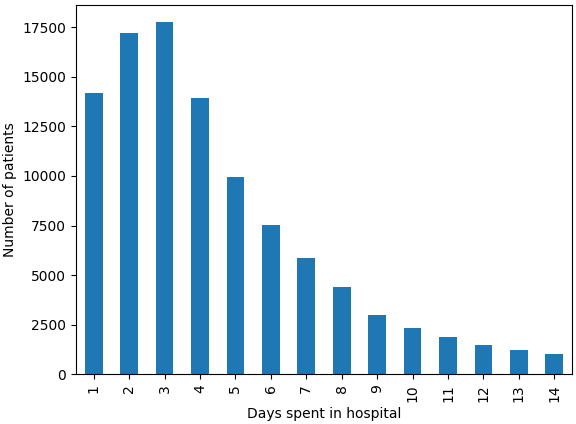
\includegraphics[width=1\textwidth]{tih_hist.png}
	\caption{Days spent in hospital per patient}
	\end{minipage}
	\hfill
	\begin{minipage}[b]{.5\textwidth}
	\centering
	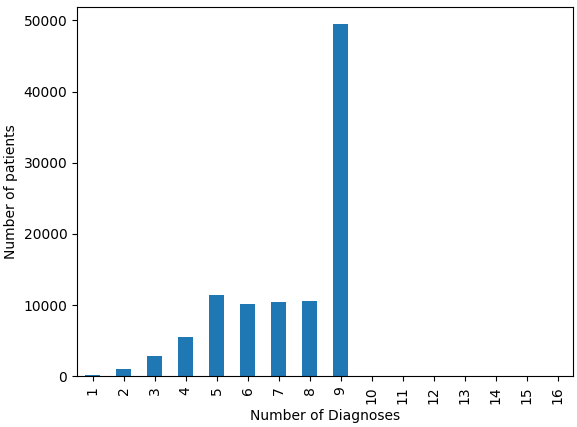
\includegraphics[width=1\textwidth]{nod_bar.png}
\caption{Diagnoses per patient}
\end{minipage}
\end{figure}

\noindent
From Figure 1 we can observe that most patients stay in the hospital between 1 and 4 days, from this we can also see that there is positive skewness. Furthermore, from Figure 2 we can observe that most patients have 9 diagnoses (almost 50\% of patients), however there are many patients that have less than 9 and rarely any patients that exceed 9 number of diagnoses. This shows that most patients had 9 diagnoses which may include diseases, injuries or any other symptom that was entered onto the system \cite{table2}. We can also make a confident assertion that a higher number of diagnoses will result in higher chance of a patient being readmitted to the hospital due to the nature of these diagnoses. It may directly correlate to the probability of readmissions.

\linespace
A scatter plot matrix enables us to visualize correlations between well-specified columns. This is useful to see how the different columns are related to each other in the data we have. 


\begin{figure}[h!]
  \centering
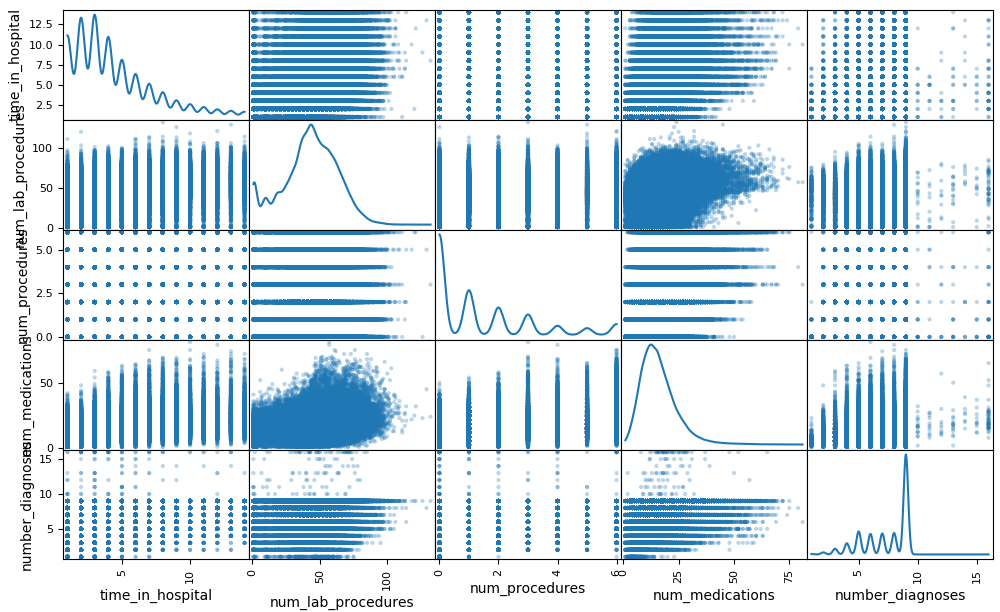
\includegraphics[width=1\textwidth]{combined_matrix.png}
  \caption{Scatter plot matrix showing correlations between numeric columns}
\end{figure}

\linespace
We do not see much correlation between our selected columns in the matrix, this could be due to the scaling of the different variables which is more than likely. For example a patient might take 5 medications but has 1 diagnosis, on the other hand another patient might take 5 medications but has 9 diagnoses. We can analyse the data further and make evaluations to help us as the matrix is not very useful in this case. 

\linespace
At a basic level we can visualise the proportion of diabetic patients by race and gender, the results of this can be seen below.

\begin{figure}[ht]
	\begin{minipage}[b]{.4\textwidth}
	\centering
	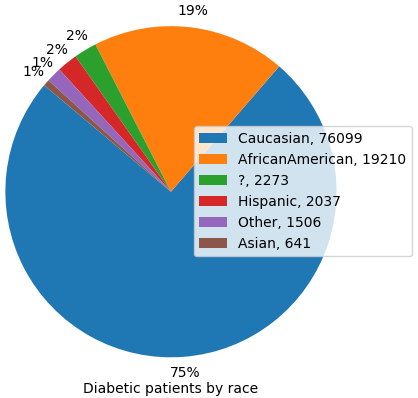
\includegraphics[width=0.8\textwidth]{race_pie.png}
	\caption{Proportion of patients by race}
	\end{minipage}
	\hfill
	\begin{minipage}[b]{.4\textwidth}
	\centering
	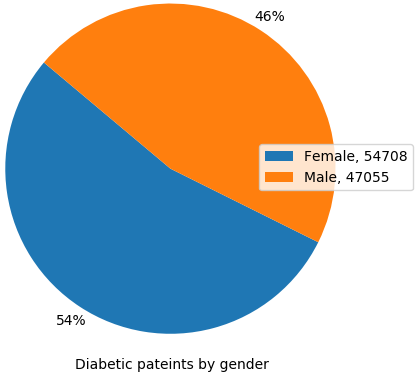
\includegraphics[width=0.8\textwidth]{gender_pie.png}
\caption{Proportion of patients by gender}
\end{minipage}
\end{figure}

\

\linespace
From this we can see that majority of diabetic patients admitted to US hospitals from 1999 to 2008 are mostly Caucasian (75\%). By analysing the gender split, it's almost an equal split however a higher percentage of females (54\%) than males (46\%). By looking at the ethnicity and gender features, we can confidently make the assertion that it does \textbf{not} motivate whether or not a patient is likely to be readmitted to the hospital. It does not provide us with any information as to whether a Caucasian male is more likely to be readmitted for diabetes than an African America female, for example. Thus, it may not be productive to consider these features in our model for predicting if a patient will be readmitted. 

\linespace
In the data-set there is some confusion between the type of readmission, where values are either ``NO'' ``\texttt{<30}'' or ``\texttt{>30}''. To avoid this confusion we can simply say that any value which is not ``NO'' is ``YES'' as we don't require any other information to make predictions. We can further observe the admission type of a patient and whether they have been readmitted to a hospital. Below the figures show the proportion of readmitted patients in the data-set and also the admission distribution.

\begin{figure}[ht]
	\begin{minipage}[b]{.4\textwidth}
	\centering
	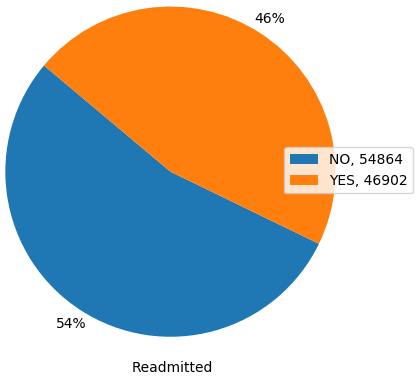
\includegraphics[width=1\textwidth]{readmitted_pie.png}
	\caption{Proportion of diabetics by race}
	\end{minipage}
	\hfill
	\begin{minipage}[b]{.4\textwidth}
	\centering
	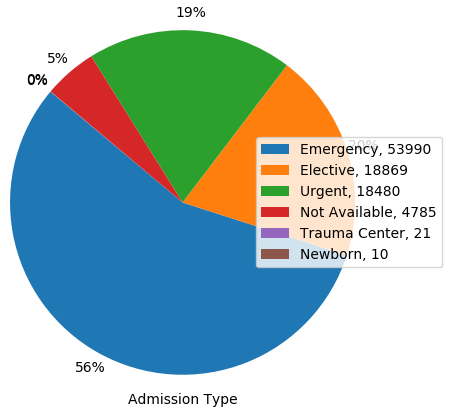
\includegraphics[width=1\textwidth]{admission_type_pie.png}
\caption{Proportion of diabetics by gender}
\end{minipage}
\end{figure}

\noindent
From this we can see that \textit{about} half of the patients are readmitted to the hospital and in most cases the reason for the admission is Emergency.

\newpage
\section{Analysing impacts of variables}

\noindent
It's very important for us to consider the impacts of the different variables in our data to the goal we have set in order to make a prediction. For this we can use box-plot which give us a good idea of how many outliers there are and what the tails and distribution of the numerical data look like in our data-set.

\linespace
For this we will analyse the following:

\begin{itemize}
	\itemsep0em 
	\item Number of emergencies
	\item Number of medications
	\item Number of Procedures
	\item Number of diagnoses
\end{itemize}

After analysing these variables in our data-set we observe the following results:


\begin{figure}[!h]
   \begin{minipage}{\textwidth}
     \centering
     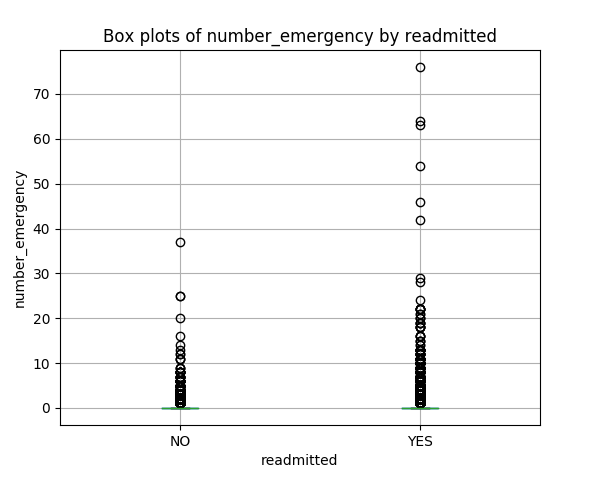
\includegraphics[width=.45\textwidth]{bplot_emergency.png}\quad
     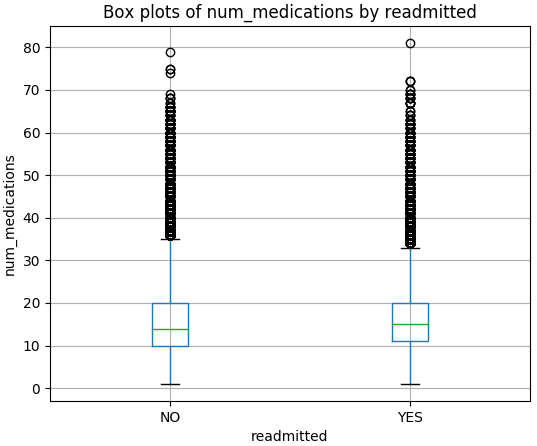
\includegraphics[width=.45\textwidth]{bplot_meds.png}\\
     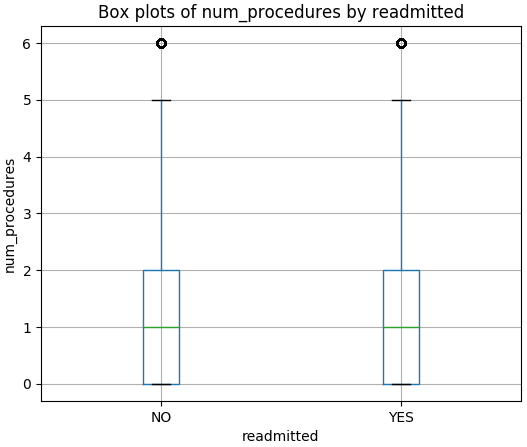
\includegraphics[width=.45\textwidth]{bplot_proc.png}\quad
     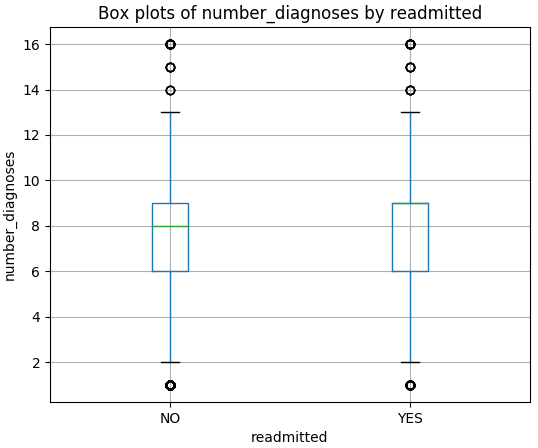
\includegraphics[width=.45\textwidth]{bplot_diag.png}
     \caption{Box plots of the above observations}
   \end{minipage}\\[1em]
  
\end{figure}
\noindent
From Figure 7 we notice that there are many \textit{suspected} outliers in our variables. For instance, observing the \texttt{num\_medications} variable we can see that there are many outlying values after the tails, similarly we can notice this for \texttt{number\_emergency}. To make an improvement to this we can \textbf{remove the outlying values} from our data-set using a $z\mathrm{-score}$ measure. To do this we can use the following equation: 

\begin{myeq}
z_{i} =  \frac{ x_{i}  -  \overline{x}}{S} 	
\end{myeq}

\noindent
In python this is much simpler by using \texttt{scipy.stats.zscore} which is able to calculate the $z\mathrm{-score}$ values for a given DataFrame. After applying this method to our data-set we can observe the following box-plots.

\begin{figure}[!ht]
   \begin{minipage}{\textwidth}
     \centering
     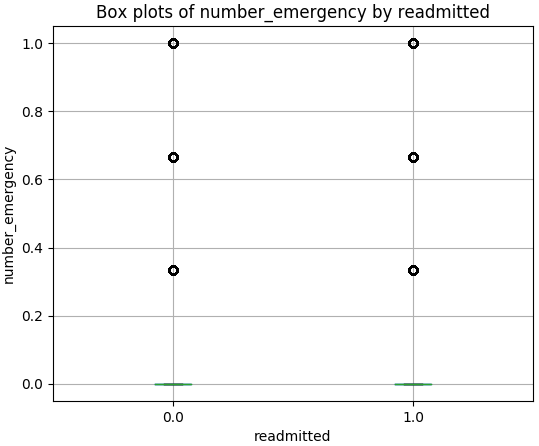
\includegraphics[width=.45\textwidth]{bplot_out_emergency.png}\quad
     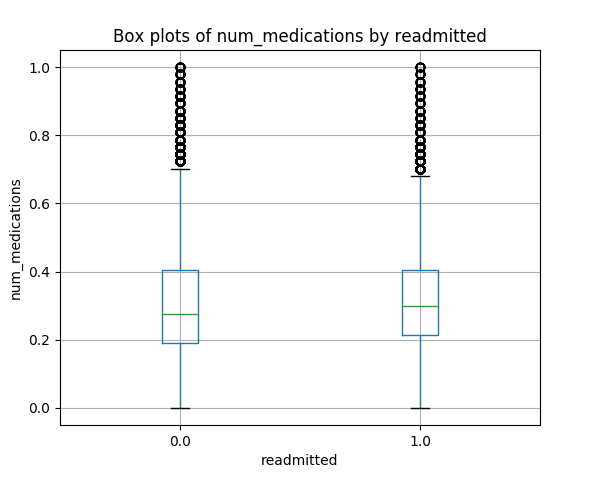
\includegraphics[width=.45\textwidth]{bplot_out_meds.png}\\
     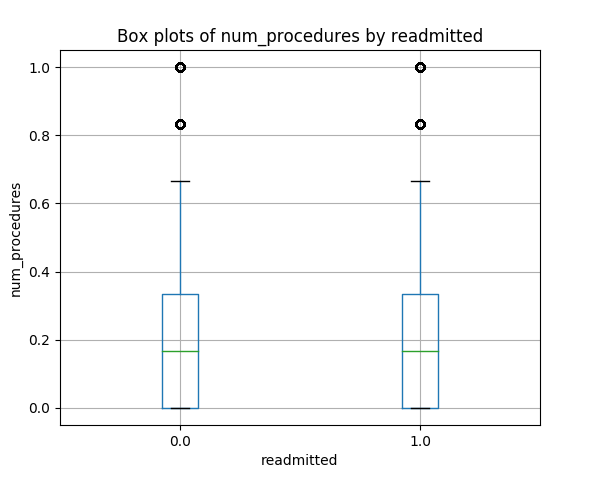
\includegraphics[width=.45\textwidth]{bplot_out_proc.png}\quad
     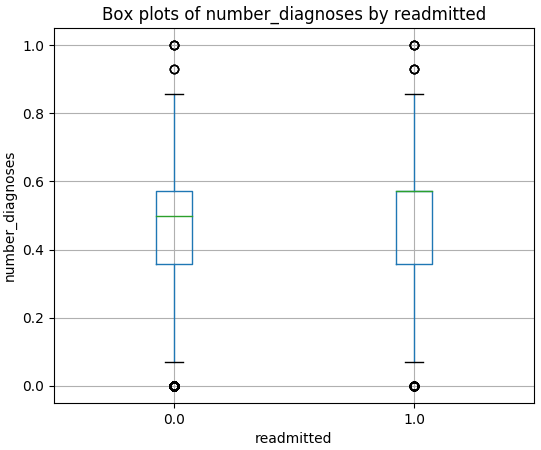
\includegraphics[width=.45\textwidth]{bplot_out_diag.png}
     \caption{Box plots of the above observations removing outliers}
   \end{minipage}\\[1em]
  
\end{figure}

\noindent
From Figure 8 we can observe that specifically for \texttt{number\_emergency} and \texttt{num\_medications} we have made a vast improvement in removing most of the outliers. It is important that we make these observations as it contributes heavily to the predictive model that we are aiming to create because it eliminates biased examples. Furthermore, we have normalised this data-set so now we can perform clustering to get more insight into the data-set.

\linespace
It is rather important to clarify that removing outliers in the data \textit{could} be dangerous because we are removing information which will be used to make predictions. For instance, we might think that a value is outlying, however when we visualise the data we might find that the outliers in fact help us make conclusions about the data such as trends, or statistical analysis such as analysing quartiles or standard deviations. In the context of this study it is even more important that we are careful with the information as we are working in a medical context which is a very sensitive area in the real world, so if this approach of removing outliers was to be used in practice, it may be more harmful. 

\clearpage
\section{Clustering}

\noindent
Before we can begin making predictions on our data-set it is important that we perform clustering, this will indicate what variables in our data-set can be observed and the impact it will have on making predictions. To do this we will use K-Means clustering.

\linespace
It should be noted that evaluating the quality of our clusters is very difficult but we should be able to form clusters that make sense in the context of our data-set. 

\subsection{K-Means Clustering}
K-Means is a type of unsupervised learning approach in which our aim is to find groups of data and their correlation to get a better insight into the information we have. 

\linespace
Our goal with K-Means clustering is as follows (to be minimised):

\begin{myeq}
cost(c_{1}, c_{2}, ..., c_{n}) =   \sum_i \underset{k}{min}(dist(x_{i}, c_{k}))
\end{myeq}

\noindent
The standard K-Means algorithm isn't directly applicable to categorical data, for various reasons. The sample space for categorical data is discrete, and doesn't have a natural origin. We can only apply the euclidean distance function to relevant data, i.e. data that is numeric. So in this case we can only find clusters for numerical columns which we feel are necessary to compare.

\begin{figure}[!ht]
   \begin{minipage}{\textwidth}
     \centering
     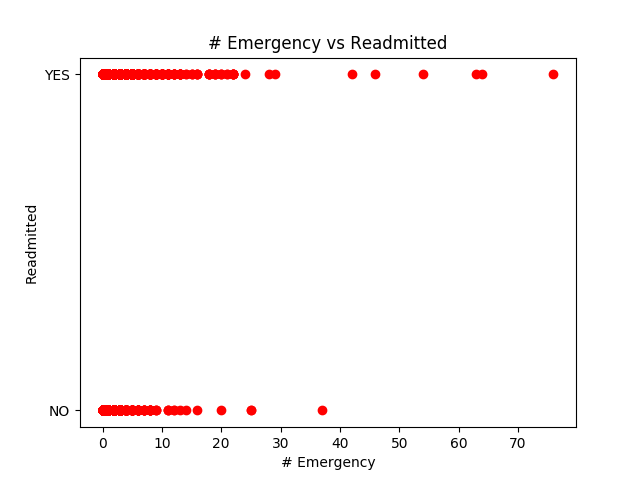
\includegraphics[width=.4\textwidth]{emergency_clust.png}\quad
     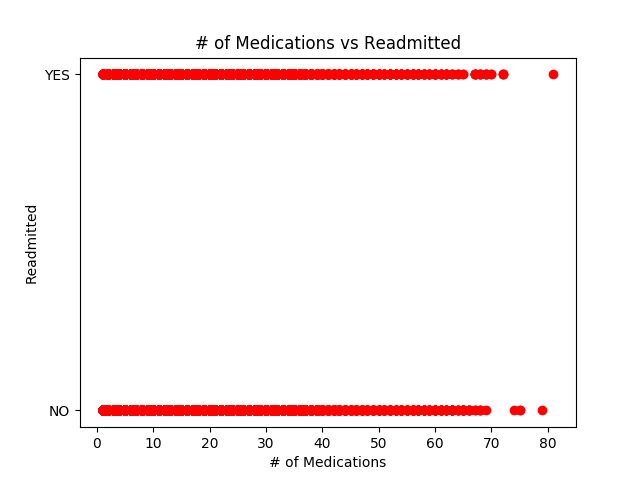
\includegraphics[width=.4\textwidth]{meds_clust.png}\\
     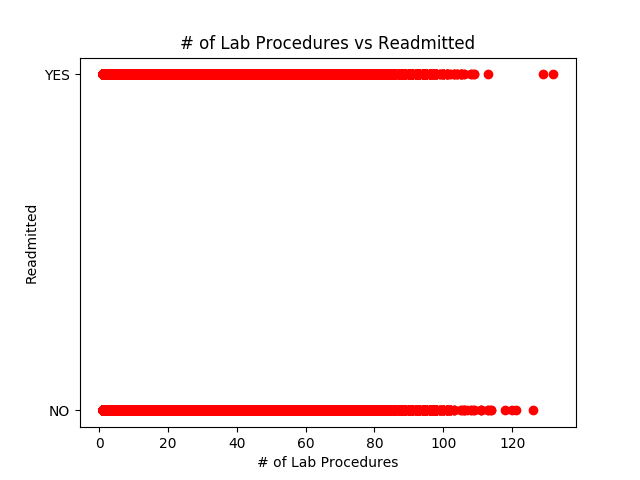
\includegraphics[width=.4\textwidth]{proc_clust.png}\quad
     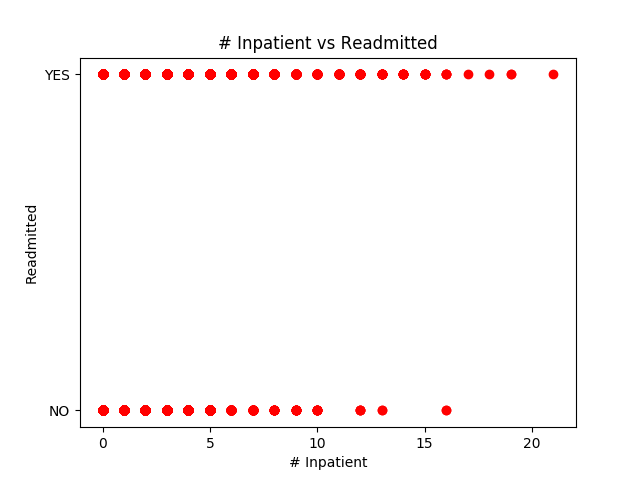
\includegraphics[width=.4\textwidth]{inpatient_clust.png}
     \caption{Clusters of relevant numeric columns vs predicted column}
   \end{minipage}\\[1em]
\end{figure}

\noindent
From the above we can see that \texttt{Emergency vs Readmitted} has a very interesting distribution and the scatter plot shows values that might be worth considering for our predictive model. The same can be observed for \texttt{Inpatient}.

\linespace
We can group the data on the \texttt{admission\_type\_id} column to give us an indication of the proportionality of the readmission values, and furthermore we can also consider age and group our data on the \texttt{age} column. 

\begin{table}[!ht]
    %\caption{}
    \begin{minipage}[t]{.5\linewidth}
      \caption{Readmission grouped by type of admission}
      \centering
        \begin{tabular}{|c|c|c|}
\hline
\multirow{2}{*}{Elective}      & YES & 7707  \\ 
                               & NO  & 11162 \\ \hline
\multirow{2}{*}{Emergency}     & YES & 25530 \\
                               & NO  & 28460 \\ \hline 
\multirow{2}{*}{Newborn}       & YES & 3     \\
                               & NO  & 7     \\ \hline
\multirow{2}{*}{Not Available} & YES & 2216  \\
                               & NO  & 2569  \\ \hline 
\multirow{2}{*}{Trauma Center} & YES & 0     \\
                               & NO  & 21    \\ \hline
\multirow{2}{*}{Urgent}        & YES & 8518  \\
                               & NO  & 9962  \\ \hline
\end{tabular}
    \end{minipage}%
    \begin{minipage}[t]{.5\linewidth}
      \centering
        \caption{Readmission grouped by type of age}
        \begin{tabular}{|c|c|c|}
\hline
\multirow{2}{*}{[0-20)}        & YES & 293   \\
                               & NO  & 559   \\ \hline 
\multirow{2}{*}{[20-40)}       & YES & 5357 \\
                               & NO  & 3075   \\ \hline
\multirow{2}{*}{[40-60)}       & YES & 11890     \\
                               & NO  & 15051    \\ \hline
\multirow{2}{*}{[60-80)}       & YES & 22943  \\
                               & NO  & 25608  \\ \hline
\multirow{2}{*}{[80-100)}       & YES & 9419  \\
                               & NO  & 14219  \\ \hline
\end{tabular}
    \end{minipage} 
\end{table}

\noindent
In Table 1 we can notice that a lot of the patients are admitted for ``Emergency'', and some as ``Elective''. We can also see that almost 50\% of patients who are admitted for ``Emergency'' are readmitted at some point. From this we can confidently assert that the type of admission may be very important in predicting whether a patient is likely to be readmitted at some point. The same assertion can be made about age, we can see that in regards to age-group, patients that are older are admitted more frequently and this increases the chance of them being readmitted at some point.

\linespace
We can further visualise our clusters using a histogram to see what clusters we can use in grouping the data and what will help us decide the variables to pick in making predictions later on.

\begin{figure}[ht]
	\begin{minipage}[b]{.5\textwidth}
	\centering
	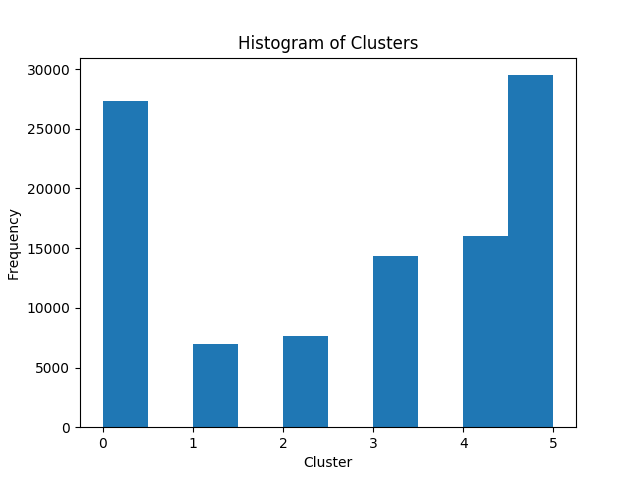
\includegraphics[width=1\textwidth]{clust_hist.png}
	\caption{K-Means - Histogram visualisation}
	\end{minipage}
	\hfill
	\begin{minipage}[b]{.5\textwidth}
	\centering
	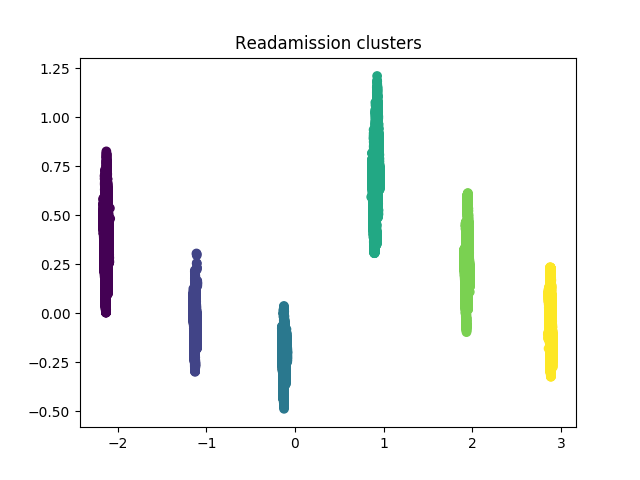
\includegraphics[width=1\textwidth]{clust_scatter.png}
\caption{K-Means - Scatter plot visualisation}
\end{minipage}
\end{figure}
\noindent
From Figure 11, we can see that we have 4 clusters with \textit{good} frequencies, showing that there is some groups that might be worth analysing. In the histogram we are looking for a \textit{uniform} distribution but we will still gain information with the results we have obtained. Furthermore from Figure 12 we can visualise the clusters and see the relationship of the clusters, we can see that the distribution of these clusters is fairly similar to the histograms we produced.

\subsection{J-Score}

The goal of this algorithm is to attain a configuration of cluster centers and cluster data
points so that the overall
J-squared error function or J-score is minimized \cite{W7Lectures}

\begin{myeq}
\displaystyle
J = \sum_{n=1}^{k} \sum_{j=1}^{C_{i}} dist(X_{j}, c_{i})^2
\end{myeq}

\noindent
Where, $dist$ is the distance, $k$ is number of clusters, $C_{i}$ the number of points in the cluster, and $c_{i}$ is the centroid of the $i^{th}$ cluster. 

\linespace
When we run a J-Score function to measure our clustering on our data-set we obtain the following values:

\begin{lstlisting}
J-score =  6935.49978087638
  score =  -6935.499780876384
\end{lstlisting}
\noindent
J-Score or \textit{inertia} is sensitive to many factors such as scale, values, number of clusters etc. So it is rather difficult to measure if this is a good score or not, but we have to rely on luck in most cases or we can keep trying more runs of the K-Means clustering process to see if we notice any improvements.

\subsection{Thresholds} 

In thresholding we aim to find the probability of predicting the clusters and the accuracy of the predictions we are making. Though thresholds don't give us accurate results and using the right method of thresholding is difficult to find, we can simply compare actual and predicted values to see what we can find. By running thresholding on our data-set we can observe the following results:

\begin{lstlisting}
Threshold0.2:           Threshold0.3:          Threshold0.5:
predict     1    		   predict    0     1     predict     0     1 
actual           		   actual                 actual
1.0      4010    		   1.0      274  3        1.0      2900  1110
2.0      3184    		   2.0      230  2954     2.0      2307   877

Threshold0.1:           Threshold0.01:          Threshold0.08:
predict     1           predict     1           predict     1
actual                  actual                  actual       
1.0      4010           1.0      4010           1.0      4010
2.0      3184           2.0      3184           2.0      3184
\end{lstlisting}


\newpage
\section{Predictive Model}
\noindent
Now that we have enough information as to what columns we should use to make predictions, we can start to create a predictive model and measure the accuracy of how well it will perform. Firstly we can try to create a \texttt{LogisticRegression} model on the numerical data that we have observed and see how it performs, this will also give us the coefficients we need to be able to make a prediction. The reason for the use of Logistic Regression is because we have many independent variables in our data-set to form a prediction from, the goal with this method would be to find the best relationships characters of interest to base a prediction from. 

\begin{lstlisting}
Model score:
	0.6130268199233716
Intercept:
	[-1.25150931]
	
Coefficients:
number_emergency     : 0.31172740417989425
time_in_hospital     : 0.012366242571301056
num_lab_procedures  : 0.0013333635661691681
num_procedures       : -0.04717337377718011
num_medications      : 0.007006666815777631
number_diagnoses     : 0.08161611884097436
number_inpatient     : 0.4204984706176172
number_outpatient    : 0.15157379083560946
\end{lstlisting}
\noindent
From this we observe a model score of \texttt{0.61} which is fairly good considering we are only using numerical values. We can further use an ROC curve to see how our model The ROC curve is created by plotting the true positive rate (TPR) against the false positive rate (FPR) at various threshold settings. This allows us to conduct a cost-benefit-analysis as to what information will help us get the best predictions. From this we observe the following:

\begin{lstlisting}
Mean hits: 0.5645594498128372
Accuracy score: 0.5645594498128372
Cross validation mean scores: 0.5798723814459725
AUC = 0.584590174618275
\end{lstlisting}

\noindent
Here we observe an AUC value of 0.58 which is very low. To improve this we can convert some of our categorical values into \textit{dummy} values where we are able to convert the categorical values into numeric dummy values. This will give our model more information to work with and hence we should expect a better score. 

\begin{lstlisting}
Mean hits: 0.6155584670815591
Accuracy score: 0.6155584670815591
Cross validation mean scores: 0.6146064505640898
AUC = 0.6538034645695068
\end{lstlisting}

\noindent
We are now able to get a much better score from our model by considering the relevant categorical values. This is important in order to make better predictions. We can also compare the ROC curves from before and after to notice this change.

\linespace
Notice that the curve in Figure 12 is not as smooth and the area underneath is lower than the curve in Figure 13. This shows us that there is significant change due to the columns that we are considering in our predictive model. 
\newpage
\begin{figure}[ht]
	\begin{minipage}[b]{.5\textwidth}
	\centering
	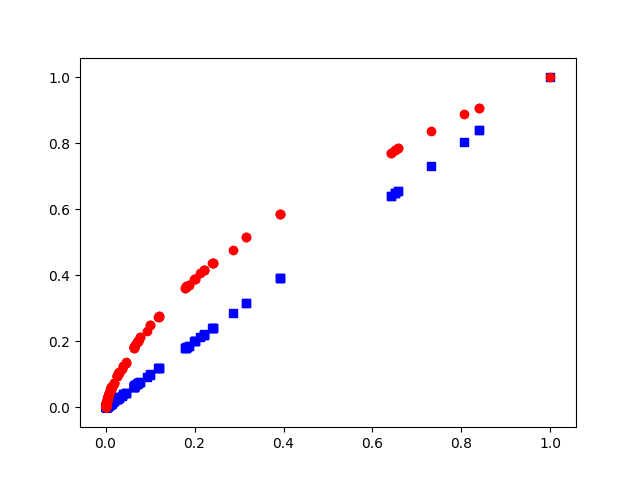
\includegraphics[width=1\textwidth]{roc_curve.png}
	\caption{ROC - only numerical columns}
	\end{minipage}
	\hfill
	\begin{minipage}[b]{.5\textwidth}
	\centering
	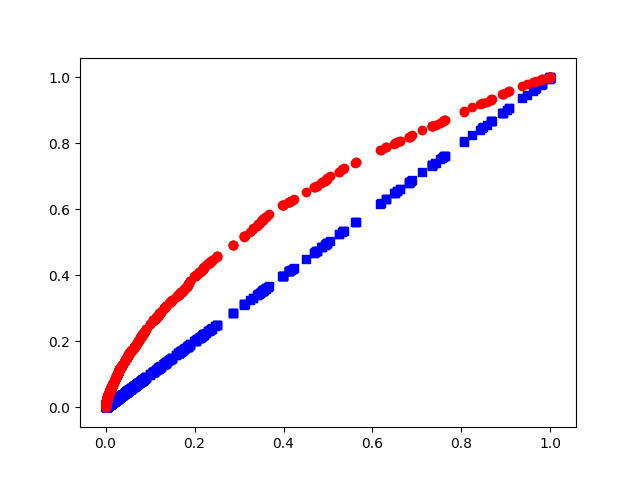
\includegraphics[width=1\textwidth]{roc_mixofnumcat.png}
\caption{ROC - categorical and numerical columns}
\end{minipage}
\end{figure}

\linespace
This model is currently using RFE or Recursive Feature Elimination in order to select the best features, in our case we are considering 15 features to build a predictive model on. We can also consider using RFECV or Recursive Feature Elimination and Cross-Validated selection in order to see if that helps in improving our model. The difference in these two techniques is in RFE we specify the number of \textit{best} features to select whereas in RFECV the number of best features are automatically tuned, this does however mean that we will notice a change in efficiency of the model.

\linespace
After running with RFECV we can notice the following results:

\begin{lstlisting}
Mean hits: 0.6155584670815591
Accuracy score: 0.6155584670815591
Cross validation mean scores: 0.6146064505640898
AUC = 0.6538034645695068
\end{lstlisting}

\begin{figure}[h!]
  \centering
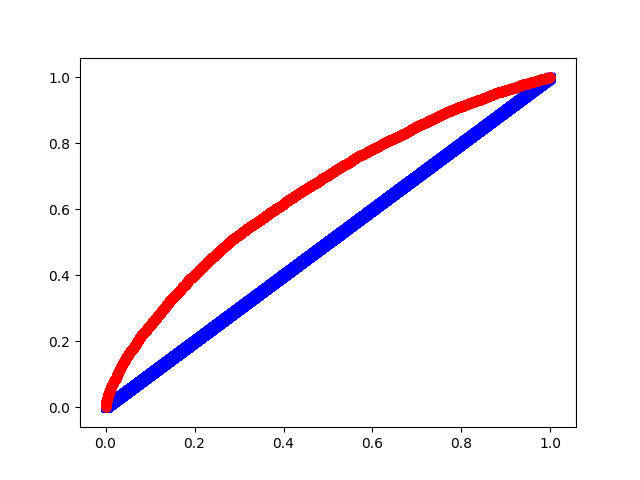
\includegraphics[width=0.5\textwidth]{rfecvroc.png}
  \caption{ROC - RFECV approach}
\end{figure}
\noindent
While this looks to be an optimistic result, we do not know what features our predictive model is using and there is not a huge change from the previous RFE approach. Thus, it would be suitable to conclude that RFE is a valid approach and we can use it for our model. 

\newpage

\section{Equation}
The final equation that we are able to obtain from our predictive model is as follows:


\begin{equation*}
\begin{aligned}
	\mathrm{Readmitted} = -1.25 + 0.312\times\mathrm{ne} + 0.012\times\mathrm{tih} + 0.001\times\mathrm{nlp} - 0.047\times\mathrm{np} + 0.007\times\mathrm{nm} \\ + 0.081\times\mathrm{nd} + 0.420\times\mathrm{ni} + 0.152\times\mathrm{no}
\end{aligned}
\end{equation*}
\noindent
Where the variables in the equation are obtained form the previous coefficients that our predictive model produced. 

\linespace
From this we can see that \texttt{ni} or \texttt{number\_inpatient} has the most effect on our prediction, i.e. a change in units will mostly be impacted by this variable. This is an important observation to make in order to understand what affects the prediction the most. We would therefore expect that a higher \texttt{ni} value will heavily affect the prediction. 

\section{Conclusion}
In this study we have looked at the data-set \texttt{Diabetes 130-US hospitals for years 1999-2008} and we have made analyses, visualisations, clustering and predictions. In essence we have been able to achieve a score of \texttt{0.65} for the area under our ROC curve and a cross-validation mean score of 0.61. While this does not look to be great, it is important to note that the score we have been able to obtain heavily relies on the data-set and missing values. There are many missing values in the data-set and in the case that we had more information it may be safe to assert that it would help in making predictions.

\linespace
It is important to reiterate that this model will most likely not be fit to use for making real world predictions but may be used as a guidance to test different features to find correlations and relationships which may give us more insight into diabetes using a linear modelling approach.

  \begin{thebibliography}{1}

  \bibitem{table2} Beata Strack, Jonathan P. DeShazo, Chris Gennings, et al., “Impact of HbA1c Measurement on Hospital Readmission Rates: Analysis of 70,000 Clinical Database Patient Records,” BioMed Research International, vol. 2014, Article ID 781670, 11 pages, 2014. doi:10.1155/2014/781670 - \url{https://www.hindawi.com/journals/bmri/2014/781670/} - Table found at: \url{https://www.hindawi.com/journals/bmri/2014/781670/tab2/}
  
    \bibitem{W7Lectures} Week 7 Lectures regarding clustering - Found at: \url{https://blackboard.le.ac.uk/bbcswebdav/pid-1659889-dt-content-rid-4527024_2/courses/CO3093/W7Lectures%20-%20Clustering%20-%20Notes.pdf}

  \end{thebibliography}

\end{document}